% WaveCatBoost methodology + conformal prediction

\subsection{Error metrics}
\begin{frame}{Error metrics}
  \centering
  Mean absolute scaled error (MASE)\par\medskip
  $N$ is the training length, $h$ is the forecast horizon, and $S=24$ hours.
  \[
    \mathrm{MASE} = \frac{N-S}{h}\,
    \frac{\sum_{t=N+1}^{N+h}|\hat Y_t-Y_t|}
         {\sum_{t=S+1}^{N}|Y_t-Y_{t-S}|}.
  \]
  The denominator measures seasonal-naive error on the training data.
\end{frame}

\subsection{Model comparison}
\begin{frame}{Model comparison}
  \centering
  PM$_{2.5}$, 1-day horizon. Lower MASE is better.\par\medskip
  \definecolor{comparisonCPCB}{HTML}{474781}
  \definecolor{comparisonIDOne}{HTML}{8D9FCA}
  \resizebox{0.94\linewidth}{!}{%
  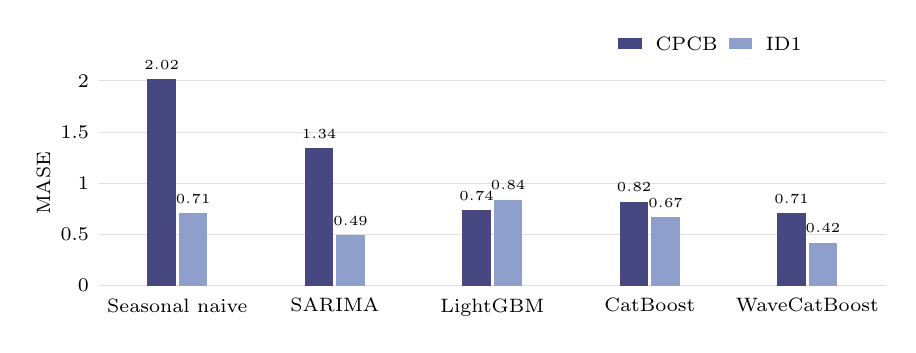
\begin{tikzpicture}[x=1cm,y=1cm,font=\scriptsize]
    \foreach \tick in {0,0.5,1,1.5,2} {
      \draw[gray!25,line width=0.3pt] (0,{1.3*\tick}) -- (10,{1.3*\tick});
      \node[left] at (0,{1.3*\tick}) {\tick};
    }
    \node[rotate=90] at (-0.7,1.3) {MASE};
    \foreach \x/\a/\b in {1/2.02/0.71,3/1.34/0.49,5/0.74/0.84,7/0.82/0.67,9/0.71/0.42} {
      \fill[comparisonCPCB] ({\x-0.38},0) rectangle ({\x-0.02},{1.3*\a});
      \fill[comparisonIDOne] ({\x+0.02},0) rectangle ({\x+0.38},{1.3*\b});
      \node[above,font=\tiny] at ({\x-0.2},{1.3*\a}) {\pgfmathprintnumber[fixed,precision=2]{\a}};
      \node[above,font=\tiny] at ({\x+0.2},{1.3*\b}) {\pgfmathprintnumber[fixed,precision=2]{\b}};
    }
    \node[below,align=center] at (1,-0.04) {Seasonal naive};
    \node[below] at (3,-0.04) {SARIMA};
    \node[below] at (5,-0.04) {LightGBM};
    \node[below] at (7,-0.04) {CatBoost};
    \node[below] at (9,-0.04) {WaveCatBoost};
    \fill[comparisonCPCB] (6.6,3.0) rectangle (6.9,3.15);
    \node[right] at (6.95,3.075) {CPCB};
    \fill[comparisonIDOne] (8.0,3.0) rectangle (8.3,3.15);
    \node[right] at (8.35,3.075) {ID1};
  \end{tikzpicture}%
  }
  \par\smallskip
  {\scriptsize
  \begin{tabular}{lrrrrr}
    \toprule
    Sensor & Seasonal naive & SARIMA & LightGBM & CatBoost & WaveCatBoost \\
    \midrule
    CPCB & 2.02 & 1.34 & 0.74 & 0.82 & \textbf{0.71} \\
    ID1 & 0.71 & 0.49 & 0.84 & 0.67 & \textbf{0.42} \\
    \bottomrule
  \end{tabular}
  }
\end{frame}

\subsection{CatBoost}
\begin{frame}{CatBoost: From Trees to Ordered Boosting}
  \small
  \textbf{1. Decision tree}
  \[
    f(x)=w_j \quad \text{if }x\in R_j
  \]
  Each leaf predicts a value.\par\smallskip
  \textbf{2. Gradient boosting}
  \[
    F_0(x)=c,\qquad
    r_i=y_i-F_{m-1}(x_i),\qquad h_m(x_i)\approx r_i
  \]
  \[
    F_m(x)=F_{m-1}(x)+\eta h_m(x),
    \qquad \eta\text{ is the learning rate.}
  \]
  \[
    h_m(x_i)\approx
    -\left.\frac{\partial L(y_i,F)}{\partial F}\right|_{F=F_{m-1}(x_i)}
  \]
  \textbf{3. Ordered boosting and symmetric trees}\par
  Ordered gradients use a model fitted on preceding observations.
  This reduces prediction shift.\par
  Same split at each depth. $2^d$ leaves, so $d=6\Rightarrow64$ leaves.
\end{frame}

\subsection{Hyperparameters}
\begin{frame}{Our Hyperparameters vs Original Paper}
  \small
  The paper followed a predefined protocol. We used a limited grid search
  to select the lag window, tree depth and learning rate.
  \medskip
  \centering
  {\scriptsize
  \begin{tabular}{lll}
    \toprule
    Parameter & Original paper & Our implementation \\
    \midrule
    Lag window ($p$) & 24 & $24,48 \rightarrow 24$ \\
    Wavelet depth ($K$) & $\lfloor\ln N\rfloor$, capped at 9 & 5 \\
    Tree depth & Default 6 & $4,6 \rightarrow 6$ \\
    Learning rate ($\eta$) & Automatic selection & $0.05,0.10 \rightarrow 0.05$ \\
    \bottomrule
  \end{tabular}
  }
  \[
    2\;(p)\times2\;(\mathrm{depth})\times2\;(\eta)
    =\boxed{8\text{ combinations}}
  \]
  \[
    \boxed{p=24,\quad \mathrm{depth}=6,\quad \eta=0.05}
  \]
  \begin{flushleft}
  \scriptsize
  Lag window: one daily cycle (24 h) versus two (48 h).\\
  Tree depth: 4 versus 6. Learning rate: 0.05 versus 0.10.\\
  Wavelet depth: $K=5$, using the energy-based choice and practical limits.
  The CPCB theoretical depth is $K=9$.\par\smallskip
  LightGBM selected the settings reused across the tree-based experiments.
  CatBoost was not independently tuned. The paper's core approach was retained.
  \end{flushleft}
\end{frame}

% ---- Conformal / uncertainty ----
\subsection{Conformal prediction}
\begin{frame}{Why conformal prediction?}
  \begin{columns}[c]
    \begin{column}{0.48\textwidth}
      \centering
      \begin{tikzpicture}[
        font=\scriptsize,
        >=Latex,
        panel/.style={draw=gray!40, rounded corners=3pt, inner sep=6pt,
                      fill=gray!3, minimum width=4.05cm}
      ]
        % ---- Panel 1: point forecast ----
        \node[panel, minimum height=1.7cm] (p1) {};
        \node[anchor=north west, font=\scriptsize\bfseries]
              at ([xshift=4pt,yshift=-4pt]p1.north west) {Point forecast};
        \draw[thick, gray!55] ([yshift=-0.22cm]p1.west) ++(0.4,0) -- ++(3.15,0);
        \coordinate (pf) at ([yshift=-0.22cm]p1.center);
        \fill[red!70!black] (pf) circle (2.5pt);
        \node[above=2pt] at (pf) {$\widehat Y_t$};
        \node[below=4pt, gray] at (pf) {``PM$_{2.5}=20$''};

        % ---- Arrow between panels ----
        \draw[-{Latex}, thick, gray!55] ([yshift=-0.18cm]p1.south) -- ++(0,-0.32);

        % ---- Panel 2: conformal band ----
        \node[panel, minimum height=2.25cm, below=0.62cm of p1] (p2) {};
        \node[anchor=north west, font=\scriptsize\bfseries]
              at ([xshift=4pt,yshift=-4pt]p2.north west) {+ conformal band};
        \fill[orange!16] ([xshift=0.72cm,yshift=-1.05cm]p2.north west)
              rectangle ([xshift=-0.42cm,yshift=0.42cm]p2.south east);
        \draw[thick, orange!70!black]
              ([xshift=0.72cm,yshift=-1.05cm]p2.north west)
              -- ([xshift=-0.42cm,yshift=-1.05cm]p2.north east);
        \draw[thick, orange!70!black]
              ([xshift=0.72cm,yshift=0.42cm]p2.south west)
              -- ([xshift=-0.42cm,yshift=0.42cm]p2.south east);
        \node[left=2pt, font=\tiny] at ([xshift=0.72cm,yshift=-1.05cm]p2.north west) {$U_t$};
        \node[left=2pt, font=\tiny] at ([xshift=0.72cm,yshift=0.42cm]p2.south west) {$L_t$};
        \coordinate (yh) at ([yshift=-0.08cm]p2.center);
        \coordinate (yt) at ([xshift=0.85cm,yshift=-0.35cm]p2.center);
        \fill[red!70!black] (yh) circle (2.5pt);
        \node[right=3pt] at (yh) {$\widehat Y_t$};
        \fill[black] (yt) circle (1.9pt);
        \node[right=2pt] at (yt) {$Y_t$};
      \end{tikzpicture}
    \end{column}
    \begin{column}{0.50\textwidth}
      {\footnotesize
      \begin{itemize}\setlength\itemsep{0.85em}
        \item \textbf{Need:} alerts need a safe range, not one risky guess.
        \item \textbf{Recipe:} use recent $|Y-\widehat Y|$ to set width ---
              large recent errors $\Rightarrow$ wider band.
        \item \textbf{No normal assumption:} AQ errors are spiky / quiet;
              conformal is distribution-free.
        \item \textbf{``95\%'':} about 95 of 100 hours, $Y_t\in[L_t,U_t]$
              (coverage).
      \end{itemize}
      }
    \end{column}
  \end{columns}
  \vspace{0.55em}
  {\footnotesize
  \centering
  From $\widehat Y_t$ alone to a band $[L_t,U_t]$ with target coverage $1-\alpha=95\%$.\par
  }
\end{frame}

\begin{frame}{Conformal formula}
  {\footnotesize
  \centering
  \renewcommand{\arraystretch}{1.35}
  \begin{tabular}{@{}r@{\hspace{0.7em}}c@{}}
    \textbf{Score}
      & $CS_t=\dfrac{|Y_t-\widehat Y_t|}{\widehat U_t}$ \\
    \textbf{Quantile}
      & $CQ_t=Q_{1-\alpha}\!\big(CS_{t-\kappa+1:t}\big)$ \\
    \textbf{Interval}
      & $PI_t=\widehat Y_t\pm CQ_t\,\widehat U_t$ \\
  \end{tabular}
  }
  \vspace{0.35em}
  {\scriptsize
  \centering
  Band edges:
  $L_t=\widehat Y_t-CQ_t\widehat U_t$,\
  $U_t=\widehat Y_t+CQ_t\widehat U_t$
  (clip $L_t\ge 0$).
  \par
  }
  \vspace{0.4em}
  \begin{columns}[T]
    \begin{column}{0.48\textwidth}
      {\footnotesize
      \begin{itemize}\setlength\itemsep{0.35em}
        \item $Y_t$, $\widehat Y_t$: truth / WaveCatBoost.
        \item $\widehat U_t$: local error scale (next slide).
        \item $CS_t$: scaled $|$error$|$ (nonconformity).
        \item $\alpha{=}0.05$ $\Rightarrow$ 95\% target.
        \item $\kappa\in\{24,168,336\}$~h (cal.\ window).
      \end{itemize}
      }
    \end{column}
    \begin{column}{0.50\textwidth}
      \begin{exampleblock}{How to use it}
        {\scriptsize
        \begin{enumerate}\setlength\itemsep{0.2em}
          \item Fit on train; residuals on a cal.\ window.
          \item Build $CS_t$; pick $\kappa$ for $\approx 95\%$ cal.\ coverage.
          \item Test: band $\widehat Y_t\pm CQ_t\widehat U_t$.
          \item Coverage $=$ share of $Y_t\in[L_t,U_t]$.
        \end{enumerate}
        }
      \end{exampleblock}
    \end{column}
  \end{columns}
\end{frame}

\begin{frame}{How $\widehat U_t$ and $CQ_t$ are computed}
  \begin{columns}[T]
    \begin{column}{0.48\textwidth}
      \begin{block}{$\widehat U_t$ --- local error scale}
        {\footnotesize
        Residual $e_t=Y_t-\widehat Y_t$.\\[0.35em]
        Default: \textbf{24-h rolling MAE}
        \[
          \widehat U_t=
          \operatorname{mean}\big(|e_{t-23}|,\ldots,|e_t|\big).
        \]
        Large recent mistakes $\Rightarrow$ large $\widehat U_t$
        $\Rightarrow$ wider band via $CQ_t\widehat U_t$.\\[0.35em]
        Multi-step test (no new $Y$ yet): freeze one robust
        $u^\star$ from calibration and reuse it.
        }
      \end{block}
    \end{column}
    \begin{column}{0.50\textwidth}
      \begin{block}{$CQ_t=Q_{1-\alpha}(CS_{t-\kappa+1:t})$}
        {\footnotesize
        \begin{enumerate}\setlength\itemsep{0.3em}
          \item Take the last $\kappa$ scores
                $CS_{t-\kappa+1},\ldots,CS_t$.
          \item Sort them.
          \item Take the $(1-\alpha)$-quantile
                ($\alpha{=}0.05$ $\Rightarrow$ $\approx$ 95th percentile).
        \end{enumerate}
        \vspace{0.25em}
        $CQ_t$ is the cutoff for a ``normal'' scaled error.\\
        Scores with $CS\le CQ_t$ fall inside
        $\widehat Y_t\pm CQ_t\widehat U_t$.
        }
      \end{block}
    \end{column}
  \end{columns}
\end{frame}

\begin{frame}{Do the intervals work? (7-day test)}
  {\footnotesize
  \textbf{Purpose:} letter-style 7-day PM$_{2.5}$ band --- does truth sit inside the
  95\% window around WaveCatBoost?
  }
  \vspace{0.3em}
  \centering
  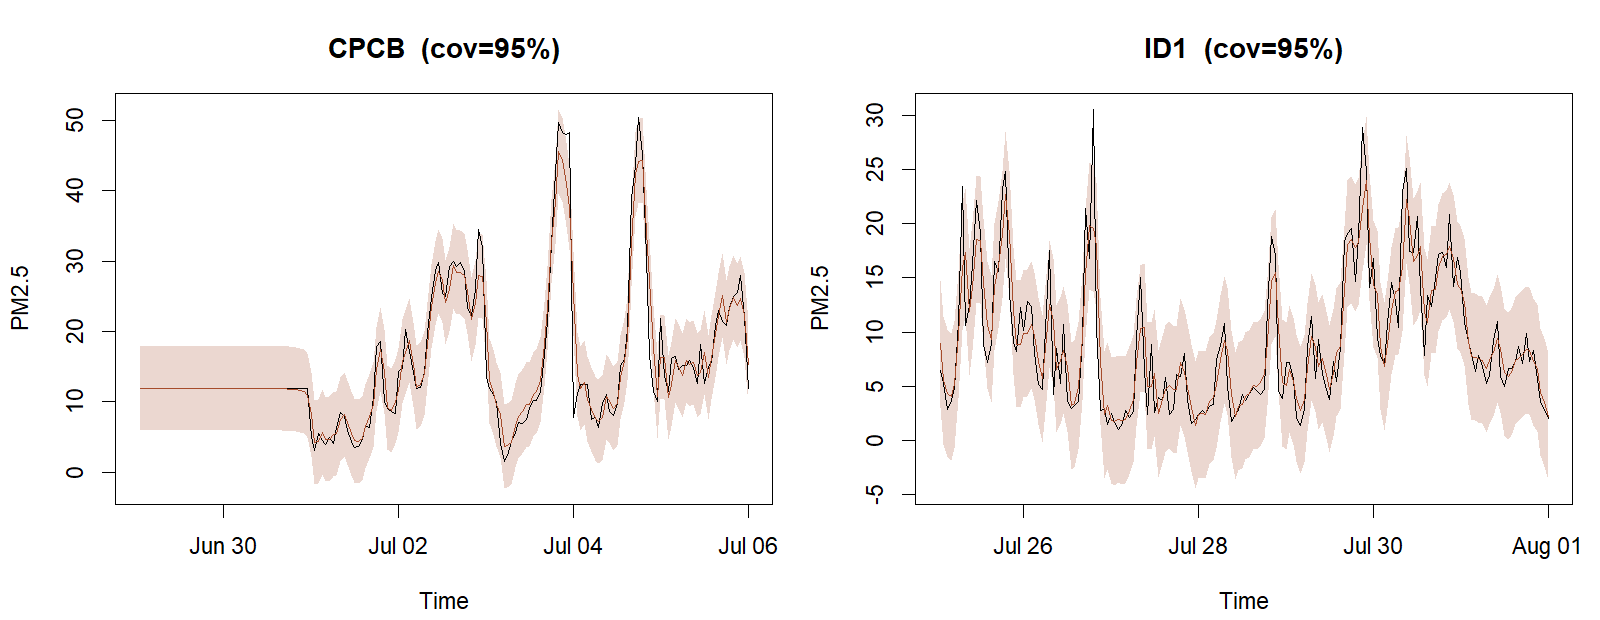
\includegraphics[width=0.98\linewidth,height=0.52\textheight,keepaspectratio]{conformal_cpcb_id1.png}
  \vspace{0.15em}
  {\footnotesize
  \begin{itemize}\setlength\itemsep{0.12em}
    \item \textbf{Black} $=$ actual;\ \textbf{orange} $=$ WaveCatBoost;\
          \textbf{shaded} $=$ 95\% residual PI $[L_t,U_t]$
          (same colours as Rmd §8.2).
    \item Paper residual PI on this window: CPCB / ID1 coverage $\approx 95\%$
          (widths $\approx 12.0$ / $11.7$).
  \end{itemize}
  }
\end{frame}

\begin{frame}{7-day paper residual PI --- summary}
  {\footnotesize
  \centering
  \begin{tabular}{lccc}
    \toprule
    Sensor & Coverage & Mean width & Point MAE \\
    \midrule
    CPCB     & 0.95 & 12.0 & 1.48 \\
    ID1      & 0.95 & 11.7 & 1.96 \\
    Shillong & 0.95 & 19.3 & 3.56 \\
    \bottomrule
  \end{tabular}
  }
  \vspace{0.7em}
  \begin{exampleblock}{Protocol}
    Rolling 1-step WaveCatBoost (letter notebook) + 95\% quantile of
    $|Y-\widehat Y|$ on the plotted 7-day window ($\alpha=0.05$).
  \end{exampleblock}
\end{frame}
